
\subsection{Discussion and Comparison of the Four methods}
\label{ssec:comparsion}

In this section we will compare the four methods in term of expressiveness, complexity, refinabilibity, and ingenuity.

\subsubsection{Ingenuity}
First we will discuss ingenuity, in other words, the design of the frameworks. The first method, GNO, relies on the Nystr\"om approximation of the kernel, or the Monte Carlo approximation of the integration. It is the most simple and straightforward method. The second method, LNO, relies on the low-rank decomposition of the kernel operator. It is efficient when the kernel has a near low-rank structure.  The third method, MGNO, is the combination of the first two. It has a hierarchical, multi-resolution decomposition of the kernel. The last one, FNO, is different from the first three;
it restricts the integral kernel to induce a convolution.

GNO and MGNO are implemented using graph neural networks, which helps to define sampling and integration. The graph network library also allows sparse and distributed message passing. The LNO and FNO don't have sampling. They are faster without using the graph library.

% GNO, LNO, and MGNO all have the kernel network $\kappa$ resembling the Green's function representation, while FNO doesn't.   FNO performs convolution on the frequency domain and it's not efficient to define the network on the frequency mode. In practice, FNO is lightweight and faster to train. \todo{I tried rewriting this paragraph but realize
% I was unsure what what being conveyed; please rewrite.}

\begin{table}[h]

\begin{center}
\begin{tabular}{l|lll}
& scheme
& graph-based
& kernel network \\  
\hline 
GNO        &  Nystr\"om  approximation & Yes   & Yes  \\
LNO       &  Low-rank approximation & No  & Yes \\
MGNO       &  Multi-level graphs on GNO & Yes   & Yes \\
FNO       & Convolution theorem; Fourier features  & No  & No \\
\hline
\end{tabular}
\end{center}
\caption{Ingenuity.}
\label{table:ingenuity}
\end{table}

\subsubsection{Expressiveness}
We measure the expressiveness by the training and testing error of the method. The full $O(J^2)$ integration always has the best results, but it is usually too expensive. As shown in the experiments \ref{ssec:DF} and \ref{ssec:BE}, GNO usually has good accuracy, but its performance suffers from sampling.
LNO works the best on the 1d problem (Burgers equation). It has difficulty on the 2d problem because it doesn't employ sampling
to speed-up evaluation. MGNO has the multi-level structure, which gives it the benefit of the first two. Finally, FNO has overall the best performance. It is also the only method that can capture the challenging Navier-Stokes equation.

% \begin{table}[h]
% \caption{Expressiveness}
% \label{table:3}
% \begin{center}
% \begin{tabular}{l|lll}
% &
% &
% & \\
% \hline 
% Nystr\"om        &   &   &  \\
% Low-rank       &   &   &  \\
% Multipole       &   &   &  \\
% Fourier       &   &   &  \\
% \hline
% \end{tabular}
% \end{center}
% \end{table}


\subsubsection{Complexity}
The complexity of the four methods are listed in Table \ref{table:complexity}. GNO and MGNO have sampling. Their complexity depends on the number of nodes sampled $J'$. When using the full nodes. They are still quadratic. LNO has the lowest complexity $O(J)$. FNO, when using the fast Fourier transform, has complexity $O(J \log J)$.

In practice. FNO is faster then the other three methods because it doesn't have the kernel network $\kappa$. MGNO is relatively slower because of its multi-level graph structure. 

\begin{table}[h]

\begin{center}
\begin{tabular}{l|cc}
& Complexity
& Time per epochs in training\\
\hline 
GNO        &  $O(J'^2 r^2)$ &  $\ 4s$ \\
LNO       &  $O(J)$ & $\ 20s$ \\
MGNO       &  $\sum_l O(J_l^2 r_l^2)  \sim O(J)$ &  $\ 8s$\\
FNO       & $(J \log J)$  &  $\ 4s$\\
\hline
\end{tabular}
\end{center}
\caption{Complexity (roundup to second on a single Nvidia V100 GPU)}
\label{table:complexity}

\end{table}

\subsubsection{Refinability}
Refineability measures the number of parameters used in the framework. Table \ref{table:refinability} lists the accuracy of the relative error on Darcy Flow with respect to different number of parameters. Because GNO, LNO, and MGNO have the kernel networks, the slope of their error rates are flat: they can work with a very small number of parameters. On the other hand, FNO does not have the sub-network. It needs at a larger magnitude of parameters to obtain an acceptable error rate.

\begin{table}[h]

\begin{center}
\begin{tabular}{l|llll}
Number of parameters
& $10^3$
&$10^4$
&$10^5$ 
& $10^6$\\
\hline 
GNO        & $\ 0.075$  & $\ 0.065$  & $\ 0.060$ & $\ 0.035$ \\
LNO       & $\ 0.080$  & $\ 0.070$  & $\ 0.060$ & $\ 0.040$ \\
MGNO       & $\ 0.070$  & $\ 0.050$  & $\ 0.040$ & $\ 0.030$ \\
FNO      & $\ 0.200$  & $\ 0.035$  & $\ 0.020$ & $\ 0.015$ \\
\hline
\end{tabular}
\caption{Refinability.}
\label{table:refinability}
\small{The relative error on Darcy Flow with respect to different number of parameters. The errors above are approximated value roundup to $0.05$. They are the lowest test error achieved by the model, given the model's number of parameters $|\theta|$ is bounded by $10^3, 10^4, 10^5, 10^6$ respectively.}
\end{center}
\end{table}



\subsubsection{Robustness}
We conclude with experiments investigating the robustness of Fourier neural operator
to noise. We study: a) training on clean (noiseless) data and testing with clean and
noisy data; b) training on clean (noiseless) data and testing with clean and
noisy data. When creating noisy data we map $a$ to noisy $a'$ as follows: 
at every grid-point $x$ we set
\[a(x)' = a(x) + 0.1 \cdot \|a\|_{\infty}\xi,\]
where  $\xi \sim \mathcal{N}(0, 1)$ is drawn i.i.d. at every grid point;
this is similar to the setting adopted in \cite{lu2021comprehensive}. 
We also study the 1d advection 
equation as an additional test case, following the setting in \cite{lu2021comprehensive}
in which the input data is a random square wave, defined by an $\R^3$-valued random
variable.


\begin{table}[h]
\begin{center}
\begin{tabular}{l|lll}
Problems
& Training error
& Test (clean)
& Test (noisy)  \\
\hline 
Burgers        & $\ 0.002$  & $\ 0.002$  & $\ 0.018$   \\
Advection        & $\ 0.002$  & $\ 0.002$  & $\ 0.094$  \\
Darcy       & $\ 0.006$  & $\ 0.011$  & $\ 0.012$  \\
Navier-Stokes       & $\ 0.024$  & $\ 0.024$  & $\ 0.039$  \\
\hline
Burgers  (train with noise)      & $\ 0.011$  & $\ 0.004$  & $\ 0.011$  \\
Advection  (train with noise)      & $\ 0.020$  & $\ 0.010$  & $\ 0.019$  \\
Darcy    (train with noise)   & $\ 0.007$  & $\ 0.012$  & $\ 0.012$  \\
Navier-Stokes   (train with noise)    & $\ 0.026$  & $\ 0.026$  & $\ 0.025$  \\
\hline
\end{tabular}\\
\end{center}
\caption{Robustness.}
\label{table:robustness}
\end{table}

As shown in the top half of Table \ref{table:robustness} and Figure \ref{fig:robustness}, we observe the Fourier neural operator is robust with respect to the (test) noise level on all four problems. In particular, on the advection problem, it has about 10\% error with 10\% noise. The Darcy and Navier-Stokes operators are smoothing, and the Fourier neural operator obtains lower than 10\% error in all scenarios. However the FNO is less robust on the advection equation, which is not smoothing, and on Burgers equation which, whilst smoothing also forms steep fronts.
%It seems the robustness of the model depends on and the dimensionality and complexity of the testing problem. For simpler and lower dimensional problem, the model overfits and loses its robustness. On the other hand, the model overfits less on the harder problem and becomes more robust. 

A straightforward approach to enhance the robustness is to train the model with noise. As shown in the bottom half of Table \ref{table:robustness}, the Fourier neural operator has no gap between the clean data and noisy data when training with noise. However, noise in training may degrade the performance on the clean data, as a trade-off. In general, augmenting the training data with noise leads to robustness. For example, in the auto-regressive modeling of dynamical systems, training the model with noise will reduce error accumulation in time, and thereby help the model to predict over longer time-horizons \citep{pfaff2020learning}.
We also observed that other regularization techniques such as early-stopping and weight decay improve robustness. Using a higher spatial resolution also helps.  

The advection problem is a hard problem for the FNO since it has discontinuities;
similar issues arise when using spectral methods for conservation laws. One can modify the architecture to address such discontinuities accordingly. For example,  \cite{wen2021u} enhance the FNO by composing a CNN or UNet branch with
the Fourier layer; the resulting composite model outperforms the basic FNO on multiphase flow with high contrast and sharp shocks. However the CNN and UNet take the method out of the realm
of discretization-invariant methods; further work is required to design
discretization-invariant image-processing tools, such as the identification of
discontinuities. 

\begin{figure}[ht]
    \centering
    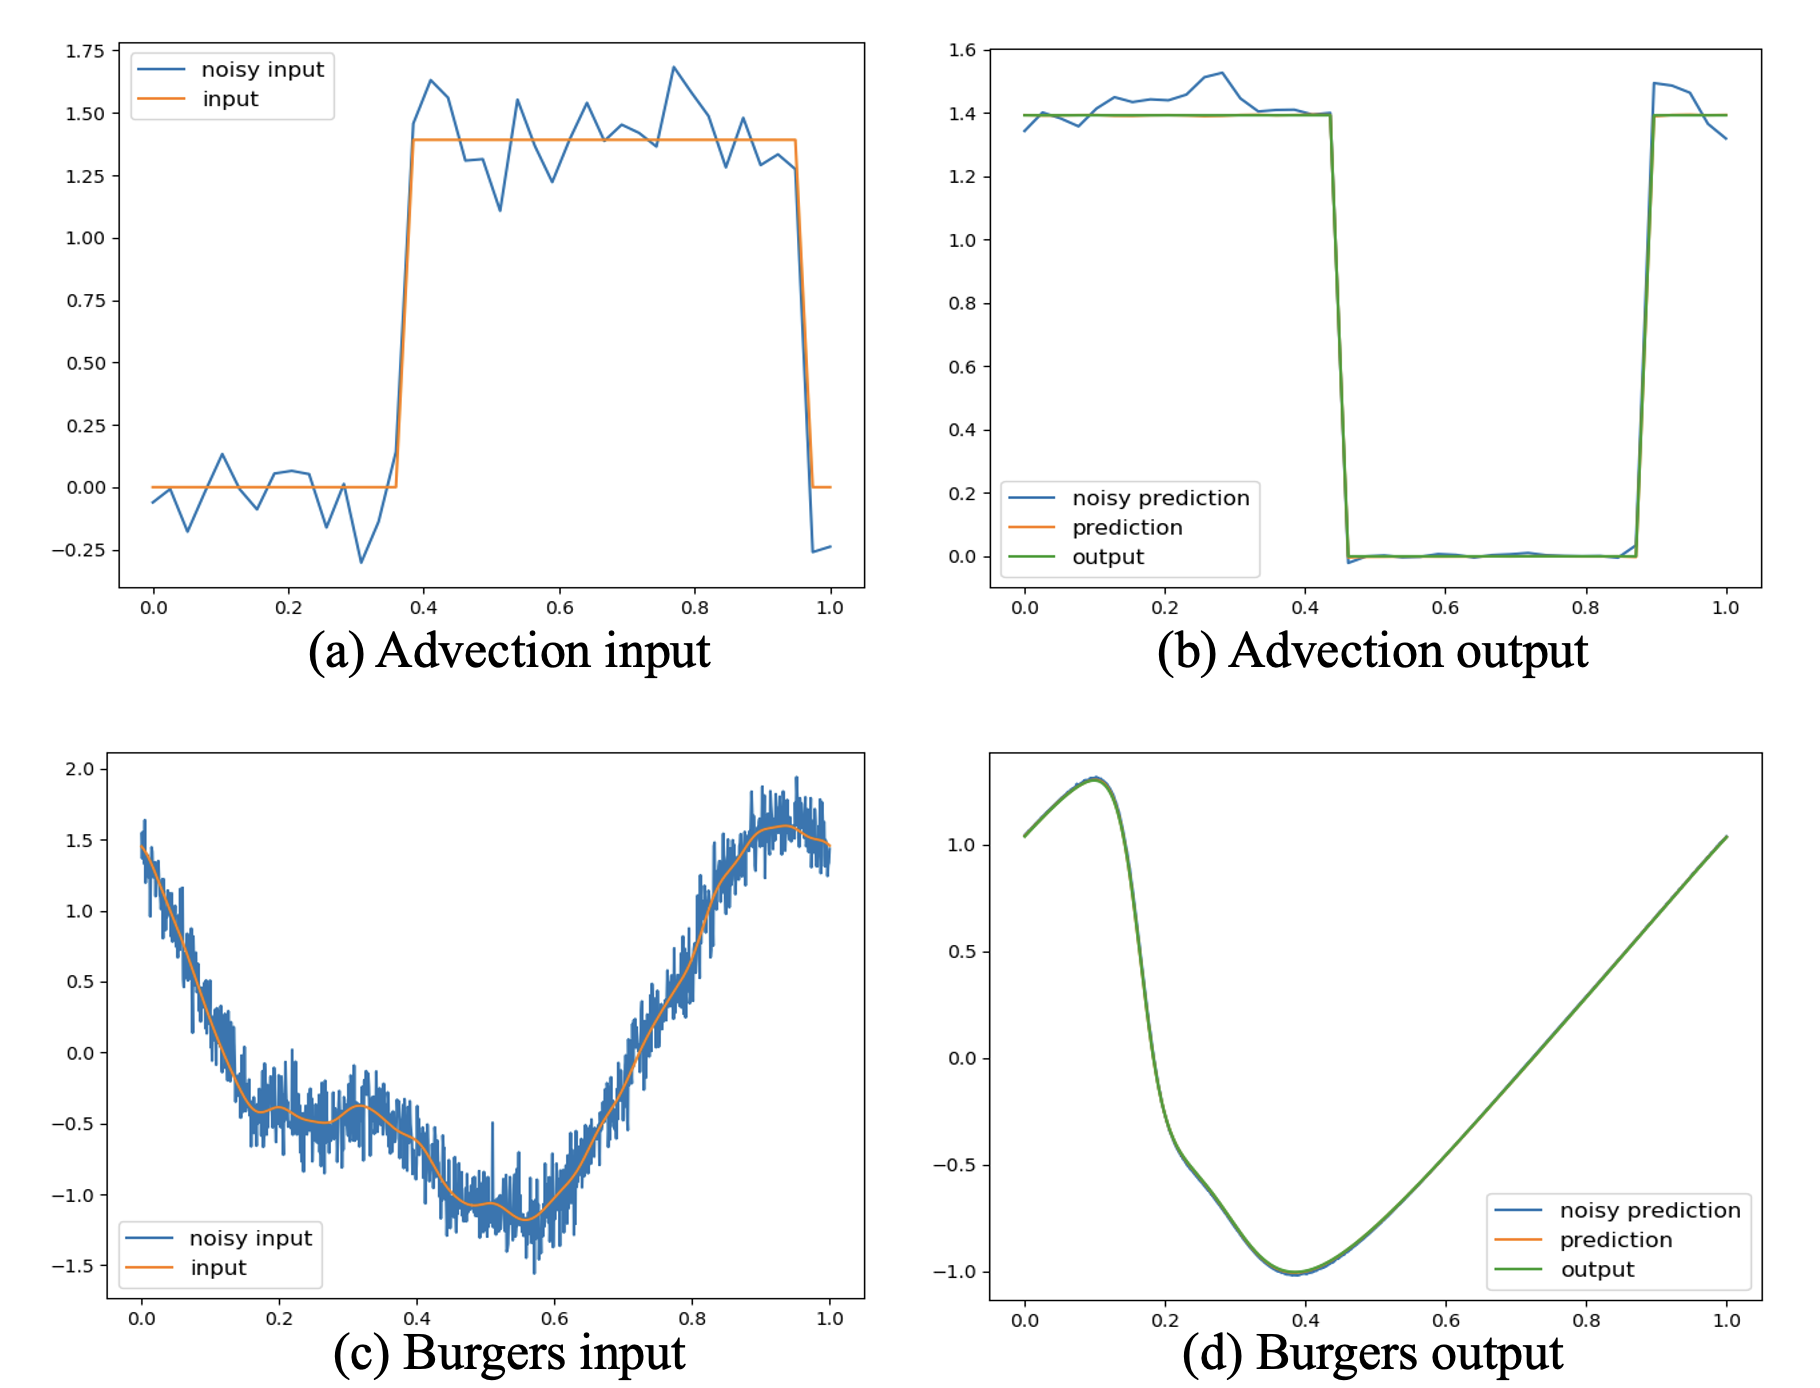
\includegraphics[width=0.7\textwidth]{Figs/robustness.png}
        \caption{Robustness on Advection and Burgers equations}\label{fig:robustness}
    \small{
    (a) The input of Advection equation ($s=40$). The orange curve is the clean input; the blue curve is the noisy input. (b) The output of Advection equation.  The green curve is the ground truth output; the orange curve is the prediction of FNO with clean input (overlapping with the ground truth); the blue curve is the prediction on the noisy input. Figure (c) and (d) are for Burgers' equation ($s=1000$) correspondingly.}
\end{figure}